\subsection{Encoders and training protocol}
\label{sec:modelos}

The models (Figure~\ref{fig:arquitetura}) project the \num{17} features $\mathbf{f}_i$ of each node onto an initial state $\mathbf{h}_i^{(0)}$ of width $D$ and apply $L = {}$\num{4} residual layers,
\begin{equation}
  \mathbf{h}_i^{(\ell)} = \mathbf{h}_i^{(\ell-1)} + \mathrm{GELU}\Big(\mathrm{Conv}^{(\ell)}\big(\mathrm{LN}^{(\ell)}(\mathbf{h}_i^{(\ell-1)}),\ \{(\mathrm{LN}^{(\ell)}(\mathbf{h}_j^{(\ell-1)}),\, \mathbf{e}_{ji})\}_{j \in \mathcal{N}(i)}\big)\Big), \quad \ell = 1, \dots, L,
  \label{eq:camada}
\end{equation}
with the layer normalisation $\mathrm{LN}^{(\ell)}$ of \citet{ba2016layer}, the GELU activation (Gaussian error linear unit) of \citet{hendrycks2016gaussian} and the operator $\mathrm{Conv}^{(\ell)}$, which reads $\mathbf{e}_{ji}$ except in EdgeConv, GraphSAGE and ResGatedGCN. In the GPS models, a learned gate mixes a local GATv2, without GELU, with global attention; a residual feed-forward block completes the layer. The readout concatenates the mean, maximum and log-compressed sum of the states. The \num{33} scalars $\mathbf{u}$ enter the regression head both directly and encoded in \num{128} dimensions. The head predicts $x$, then $y$ given the predicted $x$, and $z$ given the predicted $x$ and $y$, also in training, by the feature-wise linear modulation (FiLM) of \citet{perez2018film} or, in the models with the cascade suffix, by concatenation; the suffix designates only the head. A leaky clamp keeps the prediction inside the box \textpm(\num{6.03},~\num{6.67},~\num{29.93})\,\unit{\m}, with a small slope outside it.

\begin{figure}[H]
  \centering
  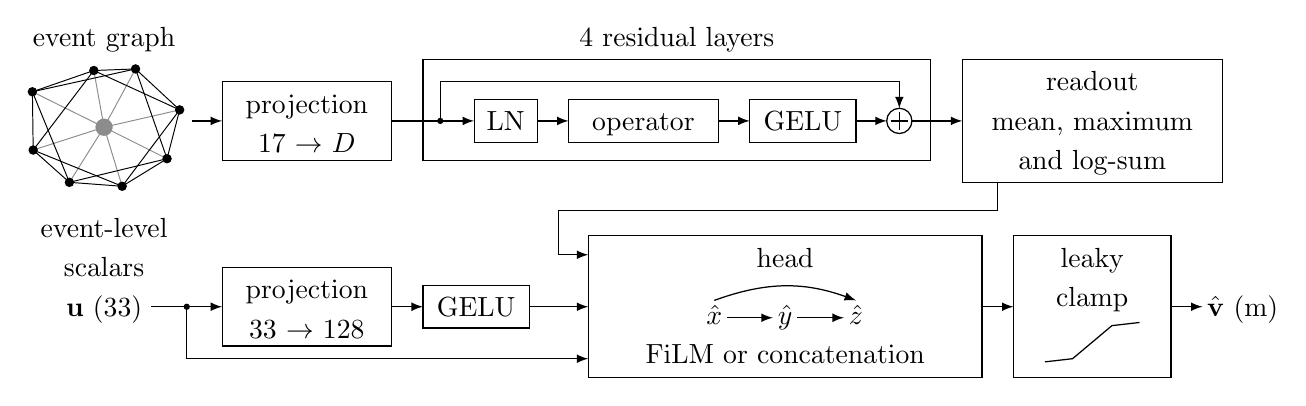
\begin{tikzpicture}[
  x=1cm, y=1cm,
  line width=0.45pt,
  flow/.style={-latex, line width=0.45pt},
  knn/.style={line width=0.35pt},
  spoke/.style={line width=0.35pt, draw=black!45},
  channel/.style={circle, fill=black, inner sep=0pt, minimum size=1.2mm},
  globalnode/.style={circle, fill=black!45, inner sep=0pt, minimum size=2.2mm},
  branch/.style={circle, fill=black, inner sep=0pt, minimum size=0.8mm},
  txt/.style={inner sep=0pt, anchor=base},
  dag/.style={inner sep=1.6pt, execute at begin node={\vphantom{$\hat{x}\hat{y}\hat{z}$}}}
]
\def\arqrowa{3.28}
\def\arqrowb{0.92}
\def\arqgap{2.14}
\def\arqtop{4.22}

\coordinate (g)  at (1.45, 3.20);
\coordinate (c0) at (2.41, 3.42);
\coordinate (c1) at (1.85, 3.94);
\coordinate (c2) at (1.32, 3.92);
\coordinate (c3) at (0.54, 3.65);
\coordinate (c4) at (0.55, 2.91);
\coordinate (c5) at (1.01, 2.50);
\coordinate (c6) at (1.68, 2.45);
\coordinate (c7) at (2.25, 2.80);

\foreach \i in {0,...,7} {\draw[spoke] (g) -- (c\i);}
\foreach \i/\j in {0/1,1/2,2/3,3/4,4/5,5/6,6/7,7/0,0/2,1/3,2/4,3/5,4/6,5/7,6/0,7/1} {\draw[knn] (c\i) -- (c\j);}
\foreach \i in {0,...,7} {\node[channel] at (c\i) {};}
\node[globalnode] at (g) {};
\node[txt] at (1.45, \arqtop) {event graph};

\draw[flow] (2.57, \arqrowa) -- (2.95, \arqrowa);
\draw (2.95, \arqrowa-0.50) rectangle (5.10, \arqrowa+0.50);
\node[txt] at (4.025, \arqrowa+0.10) {projection};
\node[txt] at (4.025, \arqrowa-0.40) {\num{17} $\to$ $D$};

\draw (5.50, \arqrowa-0.50) rectangle (11.95, \arqrowa+0.78);
\node[txt] at (8.725, \arqtop) {\num{4} residual layers};
\draw[flow] (5.10, \arqrowa) -- (6.15, \arqrowa);
\node[branch] at (5.72, \arqrowa) {};
\draw[flow] (5.72, \arqrowa) -- (5.72, \arqrowa+0.50) -- (11.55, \arqrowa+0.50) -- (11.55, \arqrowa+0.16);
\draw (6.15, \arqrowa-0.27) rectangle (6.95, \arqrowa+0.27);
\node[txt] at (6.55, \arqrowa-0.12) {LN};
\draw[flow] (6.95, \arqrowa) -- (7.35, \arqrowa);
\draw (7.35, \arqrowa-0.27) rectangle (9.25, \arqrowa+0.27);
\node[txt] at (8.30, \arqrowa-0.12) {operator};
\draw[flow] (9.25, \arqrowa) -- (9.65, \arqrowa);
\draw (9.65, \arqrowa-0.27) rectangle (11.00, \arqrowa+0.27);
\node[txt] at (10.325, \arqrowa-0.12) {GELU};
\draw[flow] (11.00, \arqrowa) -- (11.39, \arqrowa);
\draw (11.55, \arqrowa) circle (0.16);
\draw (11.44, \arqrowa) -- (11.66, \arqrowa);
\draw (11.55, \arqrowa-0.11) -- (11.55, \arqrowa+0.11);
\draw[flow] (11.71, \arqrowa) -- (12.35, \arqrowa);

\draw (12.35, \arqrowa-0.78) rectangle (15.65, \arqrowa+0.78);
\node[txt] at (14.00, \arqrowa+0.38) {readout};
\node[txt] at (14.00, \arqrowa-0.12) {mean, maximum};
\node[txt] at (14.00, \arqrowa-0.62) {and log-sum};

\draw[flow] (12.80, \arqrowa-0.78) -- (12.80, \arqgap) -- (7.225, \arqgap) -- (7.225, \arqrowb+0.66) -- (7.60, \arqrowb+0.66);

\node[txt] at (1.45, \arqrowb+0.88) {event-level};
\node[txt] at (1.45, \arqrowb+0.38) {scalars};
\node[txt] at (1.45, \arqrowb-0.12) {$\mathbf{u}$ (\num{33})};
\draw[flow] (2.05, \arqrowb) -- (2.95, \arqrowb);
\node[branch] at (2.50, \arqrowb) {};
\draw[flow] (2.50, \arqrowb) -- (2.50, \arqrowb-0.66) -- (7.60, \arqrowb-0.66);
\draw (2.95, \arqrowb-0.50) rectangle (5.10, \arqrowb+0.50);
\node[txt] at (4.025, \arqrowb+0.10) {projection};
\node[txt] at (4.025, \arqrowb-0.40) {\num{33} $\to$ \num{128}};
\draw[flow] (5.10, \arqrowb) -- (5.50, \arqrowb);
\draw (5.50, \arqrowb-0.27) rectangle (6.85, \arqrowb+0.27);
\node[txt] at (6.175, \arqrowb-0.12) {GELU};
\draw[flow] (6.85, \arqrowb) -- (7.60, \arqrowb);

\draw (7.60, \arqrowb-0.90) rectangle (12.60, \arqrowb+0.90);
\node[txt] at (10.10, \arqrowb+0.50) {head};
\node[dag] (xh) at (9.20, \arqrowb-0.14) {$\hat{x}$};
\node[dag] (yh) at (10.10, \arqrowb-0.14) {$\hat{y}$};
\node[dag] (zh) at (11.00, \arqrowb-0.14) {$\hat{z}$};
\draw[flow] (xh) -- (yh);
\draw[flow] (yh) -- (zh);
\draw[flow] (xh.north) to[bend left=20] (zh.north);
\node[txt] at (10.10, \arqrowb-0.72) {FiLM or concatenation};
\draw[flow] (12.60, \arqrowb) -- (13.00, \arqrowb);

\draw (13.00, \arqrowb-0.90) rectangle (15.00, \arqrowb+0.90);
\node[txt] at (14.00, \arqrowb+0.50) {leaky};
\node[txt] at (14.00, \arqrowb) {clamp};
\draw (13.40, \arqrowb-0.70) -- (13.75, \arqrowb-0.66) -- (14.25, \arqrowb-0.24) -- (14.60, \arqrowb-0.20);
\draw[flow] (15.00, \arqrowb) -- (15.40, \arqrowb);
\node[txt, anchor=base west] at (15.45, \arqrowb-0.12) {$\hat{\mathbf{v}}$ (m)};
\end{tikzpicture}\relax

  \caption{Structure shared by the \num{11} encoders. The event graph has one node per active channel and one global node at the light centroid; four residual layers update the node states, which the readout summarises as their mean, maximum and log-compressed sum; the head also receives the \num{33} event-level scalars and predicts $x$, then $y$ given the predicted $x$ ($\hat{x}$), and $z$ given $\hat{x}$ and the predicted $y$ ($\hat{y}$); the leaky clamp keeps the predicted vertex $\hat{\mathbf{v}}$, in metres, inside the box defined by the channels. The encoders differ only in the operator (in the GPS models, the whole layer), the width $D$ and, in the models with the cascade suffix, the head.}
  \label{fig:arquitetura}
\end{figure}

The width $D$ of each encoder was chosen \citep{dwivedi2023benchmarking} so that the parameter total approached that of GPS, \num{1843395}. Of the \num{14} sized encoders, \num{11} were trained (Section~\ref{sec:dificuldades}), with \num{1819019} to \num{1873531} parameters (maximum deviation of \qty{1.6}{\percent}) and $D$ from \num{132} to \num{685}, except for GPS (Table~\ref{tab:codificadores}). The matched capacity is that of the whole model: the encoder's share ranges from \qty{58.3}{\percent} (EdgeConv) to \qty{85.4}{\percent} (GPS-cascade).

The loss $\mathcal{L}$ is the mean Euclidean distance, in metres, between the predicted vertex $\hat{\mathbf{v}}_b$ and the true vertex $\mathbf{v}_b$ of the $B$ rows $b$ of the batch,
\begin{equation}
  \mathcal{L} = \frac{1}{B} \sum_{b=1}^{B} \big\lVert \hat{\mathbf{v}}_b - \mathbf{v}_b \big\rVert,
  \label{eq:perda}
\end{equation}
the same quantity as the mean 3-D error. The AdamW optimiser \citep{loshchilov2019decoupled} used moving-average coefficients of \num{0.9} and \num{0.999}, weight decay of \num{e-4} in the encoder and \num{e-5} in the head, and learning rates of \num{5e-4} and \num{5e-3}, respectively, for batches of \num{128} (\num{1.5e-4} and \num{1.5e-3} in the GPS models), with the rates multiplied by $B$/\num{128} \citep{goyal2017accurate}. The batch size $B$ was the largest power of two, up to \num{512}, that fitted in \qty{20}{\gibi\byte} during a memory probe: \num{128} for four models, \num{256} for two and \num{512} for five. Training used a linear warm-up over \num{100} optimisation steps starting from \num{0.1} times the rate, cosine annealing to \num{e-6} over \num{50} epochs \citep{loshchilov2017sgdr} and gradient-norm clipping at \num{1.0}. The test evaluation used the checkpoint with the lowest validation error; there was no mixed precision, no data augmentation beyond the mirroring and no moving average of the weights. Each encoder was trained once, with seed \num{42}, without a hyperparameter search. The training runs totalled \qty{11.42}{\hour} on a graphics processing unit (GPU) with \qty{23.98}{\gibi\byte} and took \num{5600} to \num{22250} steps: the capacity was matched, but the optimisation budget varied.
